\documentclass[11pt,addpoints,answers]{exam}

%%%%%%%%%%%%%%%%%%%%%%%%%%%%%%%%%%%%%%%%%%%
% Commands for customizing the assignment %
%%%%%%%%%%%%%%%%%%%%%%%%%%%%%%%%%%%%%%%%%%%

\newcommand{\courseNum}{10-423/10-623}
\newcommand{\courseName}{Generative AI}
\newcommand{\courseSem}{Spring 2024}
\newcommand{\courseUrl}{\url{http://423.mlcourse.org}}
\newcommand{\hwNum}{Homework 4}
\newcommand{\hwTopic}{Multi-Modal Foundation Models}
\newcommand{\hwName}{\hwNum: \hwTopic}
\newcommand{\outDate}{Mar. 13, 2024}
\newcommand{\dueDate}{Mar. 22, 2024}
\newcommand{\taNames}{Asmita, Haoyang, Tiancheng}
\newcommand{\homeworktype}{\string written+prog}
\newcommand{\overleafUrl}{}

%% To HIDE SOLUTIONS (to post at the website for students), set this value to 0: \def\issoln{0}
\providecommand{\issoln}{0}
%\providecommand{\issoln}{1}

%-----------------------------------------------------------------------------
% PACKAGES AND OTHER DOCUMENT CONFIGURATIONS
%-----------------------------------------------------------------------------

\usepackage[margin=1in]{geometry}
\usepackage{amsmath, amsfonts}
\usepackage{enumerate}
\usepackage{graphicx}
\usepackage{titling}
\usepackage{url}
\usepackage{xfrac}
\usepackage{natbib}
\usepackage{amssymb}
\usepackage{amsthm}
\usepackage{paralist}
\usepackage{epstopdf}
\usepackage{tabularx}
\usepackage{longtable}
\usepackage{multirow}
\usepackage{multicol}
\usepackage[colorlinks=true,urlcolor=blue]{hyperref}
\usepackage{algorithm}
\usepackage{algorithmicx}
\usepackage[noend]{algpseudocode}
\usepackage{float}
\usepackage{enumerate}
\usepackage{array}
\usepackage{environ}
\usepackage{times}
\usepackage{textcomp}
\usepackage{caption}
\usepackage{parskip} % For NIPS style paragraphs.
\usepackage[compact]{titlesec} % Less whitespace around titles
\usepackage[inline]{enumitem} % For inline enumerate* and itemize*
\usepackage{datetime}
\usepackage{comment}
% \usepackage{minted}
\usepackage{lastpage}
\usepackage{color}
% \usepackage{xcolor}
\usepackage[dvipsnames]{xcolor}
\usepackage[final]{listings}
\usepackage{tikz}
\usetikzlibrary{shapes,decorations}
\usepackage{framed}
\usepackage{booktabs}
\usepackage{cprotect}
\usepackage{verbatimbox}
\usepackage{multicol}
\usepackage{hyperref}
\usepackage{subcaption}
\usepackage{mathtools} % For drcases
\usepackage{cancel}
\usepackage[many]{tcolorbox}
\usepackage{soul}
\usepackage[bottom]{footmisc}
\usepackage{bm}
\usepackage{wasysym}
\usepackage{lipsum}

\usepackage{tikz}
\usetikzlibrary{arrows}
\usetikzlibrary{arrows.meta}
\usetikzlibrary{shapes.geometric}
\usetikzlibrary{positioning, arrows, automata, calc}
\usepackage{transparent}
\usepackage{tikz-cd}

%%%%%%%%%%%%%%%%%%%%%%%%%%%%%%%%%%%%%%%%%%%
% Formatting for \CorrectChoice of "exam" %
%%%%%%%%%%%%%%%%%%%%%%%%%%%%%%%%%%%%%%%%%%%

\CorrectChoiceEmphasis{}
\checkedchar{\blackcircle}

\newenvironment{checkboxessquare}{
    \begingroup
    \checkboxchar{$\Box$} \checkedchar{$\blacksquare$} % change checkbox style locally
    \begin{checkboxes}
    }{
    \end{checkboxes}
    \endgroup
    }

%%%%%%%%%%%%%%%%%%%%%%%%%%%%%%%%%%%%%%%%%%%
% Better numbering                        %
%%%%%%%%%%%%%%%%%%%%%%%%%%%%%%%%%%%%%%%%%%%

% \numberwithin{equation}{section} % Number equations within sections (i.e. 1.1, 1.2, 2.1, 2.2 instead of 1, 2, 3, 4)
% \numberwithin{figure}{section} % Number figures within sections (i.e. 1.1, 1.2, 2.1, 2.2 instead of 1, 2, 3, 4)
% \numberwithin{table}{section} % Number tables within sections (i.e. 1.1, 1.2, 2.1, 2.2 instead of 1, 2, 3, 4)

%%%%%%%%%%%%%%%%%%%%%%%%%%%%%%%%%%%%%%%%%%
% Custom commands                        %
%%%%%%%%%%%%%%%%%%%%%%%%%%%%%%%%%%%%%%%%%%
\newcommand{\blackcircle}{\tikz\draw[black,fill=black] (0,0) circle (1ex);}
\renewcommand{\circle}{\tikz\draw[black] (0,0) circle (1ex);}

\newcommand{\solo}{ \textcolor{orange}{[SOLO]} }
\newcommand{\open}{ \textcolor{blue}{[OPEN]} }


%%%%%%%%%%%%%%%%%%%%%%%%%%%%%%%%%%%%%%%%%%
% Custom commands for Math               %
%%%%%%%%%%%%%%%%%%%%%%%%%%%%%%%%%%%%%%%%%%
\newcommand{\vc}[1]{\boldsymbol{#1}}
\newcommand{\adj}[1]{\frac{\partial \ell}{\partial #1}}
\newcommand{\chain}[2]{\adj{#2} = \adj{#1}\frac{\partial #1}{\partial #2}}
\newcommand{\ntset}{test}
\newcommand{\zerov}{\mathbf{0}}
\DeclareMathOperator*{\argmin}{argmin}

% mathcal
\newcommand{\Ac}{\mathcal{A}}
\newcommand{\Bc}{\mathcal{B}}
\newcommand{\Cc}{\mathcal{C}}
\newcommand{\Dc}{\mathcal{D}}
\newcommand{\Ec}{\mathcal{E}}
\newcommand{\Fc}{\mathcal{F}}
\newcommand{\Gc}{\mathcal{G}}
\newcommand{\Hc}{\mathcal{H}}
\newcommand{\Ic}{\mathcal{I}}
\newcommand{\Jc}{\mathcal{J}}
\newcommand{\Kc}{\mathcal{K}}
\newcommand{\Lc}{\mathcal{L}}
\newcommand{\Mc}{\mathcal{M}}
\newcommand{\Nc}{\mathcal{N}}
\newcommand{\Oc}{\mathcal{O}}
\newcommand{\Pc}{\mathcal{P}}
\newcommand{\Qc}{\mathcal{Q}}
\newcommand{\Rc}{\mathcal{R}}
\newcommand{\Sc}{\mathcal{S}}
\newcommand{\Tc}{\mathcal{T}}
\newcommand{\Uc}{\mathcal{U}}
\newcommand{\Vc}{\mathcal{V}}
\newcommand{\Wc}{\mathcal{W}}
\newcommand{\Xc}{\mathcal{X}}
\newcommand{\Yc}{\mathcal{Y}}
\newcommand{\Zc}{\mathcal{Z}}

% mathbb
\newcommand{\Ab}{\mathbb{A}}
\newcommand{\Bb}{\mathbb{B}}
\newcommand{\Cb}{\mathbb{C}}
\newcommand{\Db}{\mathbb{D}}
\newcommand{\Eb}{\mathbb{E}}
\newcommand{\Fb}{\mathbb{F}}
\newcommand{\Gb}{\mathbb{G}}
\newcommand{\Hb}{\mathbb{H}}
\newcommand{\Ib}{\mathbb{I}}
\newcommand{\Jb}{\mathbb{J}}
\newcommand{\Kb}{\mathbb{K}}
\newcommand{\Lb}{\mathbb{L}}
\newcommand{\Mb}{\mathbb{M}}
\newcommand{\Nb}{\mathbb{N}}
\newcommand{\Ob}{\mathbb{O}}
\newcommand{\Pb}{\mathbb{P}}
\newcommand{\Qb}{\mathbb{Q}}
\newcommand{\Rb}{\mathbb{R}}
\newcommand{\Sb}{\mathbb{S}}
\newcommand{\Tb}{\mathbb{T}}
\newcommand{\Ub}{\mathbb{U}}
\newcommand{\Vb}{\mathbb{V}}
\newcommand{\Wb}{\mathbb{W}}
\newcommand{\Xb}{\mathbb{X}}
\newcommand{\Yb}{\mathbb{Y}}
\newcommand{\Zb}{\mathbb{Z}}

% mathbf lowercase
\newcommand{\av}{\mathbf{a}}
\newcommand{\bv}{\mathbf{b}}
\newcommand{\cv}{\mathbf{c}}
\newcommand{\dv}{\mathbf{d}}
\newcommand{\ev}{\mathbf{e}}
\newcommand{\fv}{\mathbf{f}}
\newcommand{\gv}{\mathbf{g}}
\newcommand{\hv}{\mathbf{h}}
\newcommand{\iv}{\mathbf{i}}
\newcommand{\jv}{\mathbf{j}}
\newcommand{\kv}{\mathbf{k}}
\newcommand{\lv}{\mathbf{l}}
\newcommand{\mv}{\mathbf{m}}
\newcommand{\nv}{\mathbf{n}}
\newcommand{\ov}{\mathbf{o}}
\newcommand{\pv}{\mathbf{p}}
\newcommand{\qv}{\mathbf{q}}
\newcommand{\rv}{\mathbf{r}}
\newcommand{\sv}{\mathbf{s}}
\newcommand{\tv}{\mathbf{t}}
\newcommand{\uv}{\mathbf{u}}
\newcommand{\vv}{\mathbf{v}}
\newcommand{\wv}{\mathbf{w}}
\newcommand{\xv}{\mathbf{x}}
\newcommand{\yv}{\mathbf{y}}
\newcommand{\zv}{\mathbf{z}}

% mathbf uppercase
\newcommand{\Av}{\mathbf{A}}
\newcommand{\Bv}{\mathbf{B}}
\newcommand{\Cv}{\mathbf{C}}
\newcommand{\Dv}{\mathbf{D}}
\newcommand{\Ev}{\mathbf{E}}
\newcommand{\Fv}{\mathbf{F}}
\newcommand{\Gv}{\mathbf{G}}
\newcommand{\Hv}{\mathbf{H}}
\newcommand{\Iv}{\mathbf{I}}
\newcommand{\Jv}{\mathbf{J}}
\newcommand{\Kv}{\mathbf{K}}
\newcommand{\Lv}{\mathbf{L}}
\newcommand{\Mv}{\mathbf{M}}
\newcommand{\Nv}{\mathbf{N}}
\newcommand{\Ov}{\mathbf{O}}
\newcommand{\Pv}{\mathbf{P}}
\newcommand{\Qv}{\mathbf{Q}}
\newcommand{\Rv}{\mathbf{R}}
\newcommand{\Sv}{\mathbf{S}}
\newcommand{\Tv}{\mathbf{T}}
\newcommand{\Uv}{\mathbf{U}}
\newcommand{\Vv}{\mathbf{V}}
\newcommand{\Wv}{\mathbf{W}}
\newcommand{\Xv}{\mathbf{X}}
\newcommand{\Yv}{\mathbf{Y}}
\newcommand{\Zv}{\mathbf{Z}}

% bold greek lowercase
\newcommand{\alphav     }{\boldsymbol \alpha     }
\newcommand{\betav      }{\boldsymbol \beta      }
\newcommand{\gammav     }{\boldsymbol \gamma     }
\newcommand{\deltav     }{\boldsymbol \delta     }
\newcommand{\epsilonv   }{\boldsymbol \epsilon   }
\newcommand{\varepsilonv}{\boldsymbol \varepsilon}
\newcommand{\zetav      }{\boldsymbol \zeta      }
\newcommand{\etav       }{\boldsymbol \eta       }
\newcommand{\thetav     }{\boldsymbol \theta     }
\newcommand{\varthetav  }{\boldsymbol \vartheta  }
\newcommand{\iotav      }{\boldsymbol \iota      }
\newcommand{\kappav     }{\boldsymbol \kappa     }
\newcommand{\varkappav  }{\boldsymbol \varkappa  }
\newcommand{\lambdav    }{\boldsymbol \lambda    }
\newcommand{\muv        }{\boldsymbol \mu        }
\newcommand{\nuv        }{\boldsymbol \nu        }
\newcommand{\xiv        }{\boldsymbol \xi        }
\newcommand{\omicronv   }{\boldsymbol \omicron   }
\newcommand{\piv        }{\boldsymbol \pi        }
\newcommand{\varpiv     }{\boldsymbol \varpi     }
\newcommand{\rhov       }{\boldsymbol \rho       }
\newcommand{\varrhov    }{\boldsymbol \varrho    }
\newcommand{\sigmav     }{\boldsymbol \sigma     }
\newcommand{\varsigmav  }{\boldsymbol \varsigma  }
\newcommand{\tauv       }{\boldsymbol \tau       }
\newcommand{\upsilonv   }{\boldsymbol \upsilon   }
\newcommand{\phiv       }{\boldsymbol \phi       }
\newcommand{\varphiv    }{\boldsymbol \varphi    }
\newcommand{\chiv       }{\boldsymbol \chi       }
\newcommand{\psiv       }{\boldsymbol \psi       }
\newcommand{\omegav     }{\boldsymbol \omega     }

% bold greek uppercase
\newcommand{\Gammav     }{\boldsymbol \Gamma     }
\newcommand{\Deltav     }{\boldsymbol \Delta     }
\newcommand{\Thetav     }{\boldsymbol \Theta     }
\newcommand{\Lambdav    }{\boldsymbol \Lambda    }
\newcommand{\Xiv        }{\boldsymbol \Xi        }
\newcommand{\Piv        }{\boldsymbol \Pi        }
\newcommand{\Sigmav     }{\boldsymbol \Sigma     }
\newcommand{\Upsilonv   }{\boldsymbol \Upsilon   }
\newcommand{\Phiv       }{\boldsymbol \Phi       }
\newcommand{\Psiv       }{\boldsymbol \Psi       }
\newcommand{\Omegav     }{\boldsymbol \Omega     }

%%%%%%%%%%%%%%%%%%%%%%%%%%%%%%%%%%%%%%%%%%%
% Code highlighting with listings         %
%%%%%%%%%%%%%%%%%%%%%%%%%%%%%%%%%%%%%%%%%%%

\definecolor{bluekeywords}{rgb}{0.13,0.13,1}
\definecolor{greencomments}{rgb}{0,0.5,0}
\definecolor{redstrings}{rgb}{0.9,0,0}
\definecolor{light-gray}{gray}{0.95}

\newcommand{\MYhref}[3][blue]{\href{#2}{\color{#1}{#3}}}%

\definecolor{dkgreen}{rgb}{0,0.6,0}
\definecolor{gray}{rgb}{0.5,0.5,0.5}
\definecolor{mauve}{rgb}{0.58,0,0.82}

\lstdefinelanguage{Shell}{
  keywords={tar, cd, make},
  %keywordstyle=\color{bluekeywords}\bfseries,
  alsoletter={+},
  ndkeywords={python3, python, py, javac, java, gcc, c, g++, cpp, .txt, octave, m, .tar},
  %ndkeywordstyle=\color{bluekeywords}\bfseries,
  identifierstyle=\color{black},
  sensitive=false,
  comment=[l]{//},
  morecomment=[s]{/*}{*/},
  commentstyle=\color{purple}\ttfamily,
  %stringstyle=\color{red}\ttfamily,
  morestring=[b]',
  morestring=[b]",
  backgroundcolor = \color{light-gray}
}

\lstset{columns=fixed, basicstyle=\ttfamily,
    backgroundcolor=\color{light-gray},xleftmargin=0.5cm,frame=tlbr,framesep=4pt,framerule=0pt}

\newcommand{\emptysquare}{{\LARGE $\square$}\ \ }
\newcommand{\filledsquare}{{\LARGE $\boxtimes$}\ \ }
\def \ifempty#1{\def\temp{#1} \ifx\temp\empty }


% \newcommand{\squaresolutionspace}[2][\emptysquare]{\newline #1}{#2}
\def \squaresolutionspace#1{ \ifempty{#1} \emptysquare \else #1\hspace{0.75pt}\fi}


\newcommand{\emptycircle}{{\LARGE $\fullmoon$}\ \ }
\newcommand{\filledcircle}{{\LARGE $\newmoon$}\ \ }
\def \circlesolutionspace#1{ \ifempty{#1} \emptycircle \else #1\hspace{0.75pt}\fi}
%%%%%%%%%%%%%%%%%%%%%%%%%%%%%%%%%%%%%%%%%%%
% Custom box for highlights               %
%%%%%%%%%%%%%%%%%%%%%%%%%%%%%%%%%%%%%%%%%%%

% Define box and box title style
\tikzstyle{mybox} = [fill=blue!10, very thick,
    rectangle, rounded corners, inner sep=1em, inner ysep=1em]

% \newcommand{\notebox}[1]{
% \begin{tikzpicture}
% \node [mybox] (box){%
%     \begin{minipage}{\textwidth}
%     #1
%     \end{minipage}
% };
% \end{tikzpicture}%
% }

\NewEnviron{notebox}{

\begin{tikzpicture}
\node [mybox] (box){
    \begin{minipage}{0.95\textwidth}
        \BODY
    \end{minipage}
};
\end{tikzpicture}
}

%%%%%%%%%%%%%%%%%%%%%%%%%%%%%%%%%%%%%%%%%%%
% Commands showing / hiding solutions     %
%%%%%%%%%%%%%%%%%%%%%%%%%%%%%%%%%%%%%%%%%%%
\newcommand{\solutionspace}[4]{\fbox{\begin{minipage}[t][#1][t]{#2} \textbf{#3} \solution{}{#4} \end{minipage}}}

% To HIDE SOLUTIONS, set this value to 0:
%\providecommand{\issoln}{0}
%\providecommand{\issoln}{1}

\ifthenelse{\equal{\issoln}{1}}{

% SOLUTION environment
\newenvironment{soln}{\leavevmode\color{red}\ignorespaces }{}

% QUESTION AUTHORS environment
\newenvironment{qauthor}{\leavevmode\color{blue}\ignorespaces }{}

% Question tester comment environment
\newenvironment{qtester}{\leavevmode\color{green}\ignorespaces}{}

% Question learning objective comment environment
\newenvironment{qlearningobjective}{\leavevmode\color{green}\ignorespaces}{}

}{ % ELSE

  \NewEnviron{soln}{}
  \NewEnviron{qauthor}{}
  \NewEnviron{qtester}{}
  \NewEnviron{qlearningobjective}{}

}

%% To HIDE TAGS set this value to 0:
\def\showtags{0}
%%%%%%%%%%%%%%%%
\ifcsname showtags\endcsname \else \def\showtags{1} \fi
% Default to an empty tags environ.
\NewEnviron{tags}{}{}
\if\showtags 1
% Otherwise, include solutions as below.
\RenewEnviron{tags}{
    \fbox{
    \leavevmode\color{blue}\ignorespaces
    \textbf{TAGS:} \texttt{\url{\BODY}}
    }
    \vspace{-.5em}
}{}
\fi

\newtcolorbox[]{answer_box}[1][]{
    % breakable,
    fit,
    enhanced,
    % nobeforeafter,
    colback=white,
    title=Your Answer,
    sidebyside align=top,
    box align=top,
    #1
}

%\pagestyle{fancyplain}
\lhead{\hwName{}
}
\rhead{\courseNum}
\cfoot{\thepage{} of \numpages{}}

\title{\textsc{\hwNum}
\\
\textsc{\hwTopic}
\thanks{Compiled on \today{} at \currenttime{}}\\
\vspace{1em}
} % Title


\author{\textsc{\large \courseNum{} \courseName{}}\\
\courseUrl
\vspace{1em}\\
\ifdefempty{\outDate}{}{  OUT: \outDate \\ }
\ifdefempty{\dueDate}{}{  DUE: \dueDate \\ }
  TAs: \taNames{}
}

\date{}

%%%%%%%%%%%%%%%%%%%%%%%%%%%%%%%%%%%%%%%%%%%%%%%%%
% Useful commands for typesetting the questions %
%%%%%%%%%%%%%%%%%%%%%%%%%%%%%%%%%%%%%%%%%%%%%%%%%

% This command will allow long \lstinline{} text to wrap automatically.
\sloppy

%%%%%%%%%%%%%%%%%%%%%%%%%%
% Document configuration %
%%%%%%%%%%%%%%%%%%%%%%%%%%

% Don't display a date in the title and remove the white space
\predate{}
\postdate{}
\date{}

% Don't display an author and remove the white space
%\preauthor{}
%\postauthor{}

% Question type commands
\newcommand{\sall}{\textbf{Select all that apply: }}
\newcommand{\sone}{\textbf{Select one: }}
\newcommand{\tf}{\textbf{True or False: }}




% Changes to examdoc
\qformat{\textbf{{\Large \thequestion \; \; \thequestiontitle \ (\totalpoints \ points)}} \hfill}
\renewcommand{\thequestion}{\arabic{question}}
\renewcommand{\questionlabel}{\thequestion.}

\renewcommand{\thepartno}{\thequestion.\arabic{partno}}
%\renewcommand{\partlabel}{\thequestion.\thepartno.}
\renewcommand{\partlabel}{\thepartno.}

% not working: \renewcommand{\subpartlabel}{(\thequestion.\thepartno.\thesubpart)}
% Commented after adding \question.\thepartno.
%\renewcommand{\partshook}{\setlength{\leftmargin}{0pt}}

\renewcommand{\thesubpart}{\thepartno.\alph{subpart}}
\renewcommand{\subpartlabel}{\thesubpart.}

\renewcommand{\thesubsubpart}{\thesubpart.\roman{subsubpart}}
\renewcommand{\subsubpartlabel}{\thesubsubpart.}

% copied from stack overflow, as all good things are
\newcommand\invisiblesection[1]{%
  \refstepcounter{section}%
  \addcontentsline{toc}{section}{\protect\numberline{\thesection}#1}%
  \sectionmark{#1}}

% quite possibly the worst workaround i have made for this class
\newcommand{\sectionquestion}[1]{
\titledquestion{#1}
\invisiblesection{#1}
~\vspace{-1em}
}

%%%%%%%%%%%%%%%%%%%%%%%%%%%%%%%%%%%%%%%%%%%
% New Environment for Pseudocode          %
%%%%%%%%%%%%%%%%%%%%%%%%%%%%%%%%%%%%%%%%%%%

% Python style for highlighting
\DeclareFixedFont{\ttb}{T1}{txtt}{bx}{n}{12} % for bold
\DeclareFixedFont{\ttm}{T1}{txtt}{m}{n}{12}  % for normal

\definecolor{deepblue}{rgb}{0,0,0.5}
\definecolor{deepred}{rgb}{0.6,0,0}
\definecolor{deepgreen}{rgb}{0,0.5,0}

\newcommand\pythonstyle{\lstset{
language=Python,
basicstyle=\ttm,
morekeywords={self},              % Add keywords here
keywordstyle=\ttb\color{deepblue},
emph={MyClass,__init__},          % Custom highlighting
emphstyle=\ttb\color{deepred},    % Custom highlighting style
stringstyle=\color{deepgreen},
frame=tb,                         % Any extra options here
showstringspaces=false
}}


% Python environment
\lstnewenvironment{your_code_solution}[1][]
{
\pythonstyle
\lstset{#1}
}
{}

\begin{document}
 
\maketitle 

\newcommand \maxsubs {10 }
\section*{Instructions}
\begin{itemize}

\item \textbf{Collaboration Policy}: Please read the collaboration policy in the syllabus.
\item\textbf{Late Submission Policy:} See the late submission policy in the syllabus.
\item\textbf{Submitting your work:} You will use Gradescope to submit
  answers to all questions\ifthenelse{\equal{\homeworktype}{\string written}}{}{ and code}. 

\begin{itemize}
    
    % IF NOT USING TEMPLATE: 
    % \item \textbf{Written:} You will submit your completed homework as a PDF to Gradescope. For each problem, please clearly indicate the question number (e.g. 3.2). Submissions can be handwritten, but must be clearly legible; otherwise, you will not be awarded marks.   Alternatively, submissions can be written in \LaTeX{}. You may use the \LaTeX{} source of this assignment (included in the handout .zip) as your starting point. For multiple choice / select all questions, simply write the letter(s) (e.g. A, B, C) corresponding to your chosen answer.
    % IF USING TEMPLATE: 
    \item \textbf{Written:} You will submit your completed homework as a PDF to Gradescope. Please use the provided template. Submissions can be handwritten, but must be clearly legible; otherwise, you will not be awarded marks. Alternatively, submissions can be written in \LaTeX{}. Each answer should be within the box provided. 
    %If you do not follow the template or your submission is misaligned, your assignment may not be graded correctly by our AI assisted grader. 
    If you do not follow the template, your assignment may not be graded correctly by our AI assisted grader and there will be a \textbf{\textcolor{red}{2\% penalty}} (e.g., if the homework is out of 100 points, 2 points will be deducted from your final score).
    
    \ifdefempty{\overleafUrl}{}{
    \item \textbf{\LaTeX{} Source:} \overleafUrl
    }

    \ifthenelse{\equal{\homeworktype}{\string written}}{}{
    \item \textbf{Programming:} You will submit your code for programming questions to Gradescope. There is no autograder. We will examine your code by hand and may award marks for its submission.
    }{}
   
  \end{itemize}
  
\ifthenelse{\equal{\homeworktype}{\string written}}{}{\item\textbf{Materials:} The data that you will need in order to complete this assignment is posted along with the writeup and template on the course website.}

\end{itemize}

\begin{center}
    \pointtable[v][questions]
\end{center}\clearpage

%\input{../shared/instructions_for_specific_problem_types.tex}
%\clearpage
\begin{questions}

\sectionquestion{Instruction Fine-Tuning \& RLHF}

\begin{parts}

\part[6] \textbf{Short answer:} Highlight the differences between in-context learning, unsupervised pre-training, supervised fine-tuning, and instruction fine-tuning by defining each one. Assume we are interested specifically in autoregressive large language models (LLMs) over text. Each definition must mention properties of the training examples and how they are used, and how learning affects the parameters of the model.
    \begin{answer_box}[title=Definition: in-context learning,height=4cm, width=15cm]
    \end{answer_box}
    \begin{answer_box}[title=Definition: unsupervised pre-training,height=4cm, width=15cm]
    \end{answer_box}
    \begin{answer_box}[title=Definition: supervised fine-tuning,height=4cm, width=15cm]
    \end{answer_box}
    \begin{answer_box}[title=Definition: instruction fine-tuning,height=4cm, width=15cm]
    \end{answer_box}

\clearpage
\part[3] \textbf{Ordering:} Consider a correctly defined reinforcement learning with human feedback (RLHF) pipeline. \textit{Select the correct ordering of the items below to define such a pipeline by numbering them from 1 to $N$. If two items can occur simultaneously, number them identically. To exclude an item from the ordering, number it as $0$.}
    \begin{itemize}
        \item \begin{answer_box}[title=,height=1cm,width=2cm,nobeforeafter,box align=center]  \end{answer_box}         Repeat the previous step many times.
        \item \begin{answer_box}[title=,height=1cm,width=2cm,nobeforeafter,box align=center]  \end{answer_box}         Repeat the following steps many times.
        \item \begin{answer_box}[title=,height=1cm,width=2cm,nobeforeafter,box align=center]  \end{answer_box}         From human labelers, collect rankings of samples from the language model.
        \item \begin{answer_box}[title=,height=1cm,width=2cm,nobeforeafter,box align=center]  \end{answer_box}         Collect instruction fine-tuning training examples from human labelers.
        \item \begin{answer_box}[title=,height=1cm,width=2cm,nobeforeafter,box align=center]  \end{answer_box}         Take a (stochastic) gradient step for a reinforcement learning objective.
        \item \begin{answer_box}[title=,height=1cm,width=2cm,nobeforeafter,box align=center]  \end{answer_box}         Sample a prompt/response pair from the language model.
        \item \begin{answer_box}[title=,height=1cm,width=2cm,nobeforeafter,box align=center]  \end{answer_box}         Collect prompt/response/reward tuples from human labelers.
        \item \begin{answer_box}[title=,height=1cm,width=2cm,nobeforeafter,box align=center]  \end{answer_box}         Perform supervised fine-tuning of the language model.
        \item \begin{answer_box}[title=,height=1cm,width=2cm,nobeforeafter,box align=center]  \end{answer_box}         Query the regression model for its score of an input.
        \item \begin{answer_box}[title=,height=1cm,width=2cm,nobeforeafter,box align=center]  \end{answer_box}         Perform supervised training of the regression model.
        \item \begin{answer_box}[title=,height=1cm,width=2cm,nobeforeafter,box align=center]  \end{answer_box}         Pre-train the language model.
    \end{itemize}
    

\end{parts}

\clearpage
\sectionquestion{Latent Diffusion Model (LDM)}

\begin{parts}

\part[2] \textbf{Short answer:} Why does a latent diffusion model run diffusion in a latent space instead of pixel space?
    \begin{answer_box}[title=,height=3cm, width=15cm]
    \end{answer_box}

\part \textbf{Short answer:} Standard cross-attention for a diffusion-based text-to-image model defines the queries $\Qv$ as a function of the pixels (or latent space) $\Yv \in \Rb^{m \times d_y}$, and the keys $\Kv$ and values $\Vv$ as a function of the text encoder output $\Xv \in \Rb^{n \times d_x}$.
\begin{align*}
    &&\Qv &= \Yv \Wv_q,
    &\Kv &= \Xv \Wv_k, 
    &\Vv &= \Xv \Wv_v
\end{align*}
(where $\Wv_q \in \Rb^{d_y \times d}$
and $\Wv_k, \Wv_v \in \Rb^{d_x \times d}$)
and then applies standard attention:
\begin{align*}
    \text{Attention}(\Qv, \Kv, \Vv) = \text{softmax}(\Qv \Kv^T / \sqrt{d}) \Vv
\end{align*}

Now, suppose you instead defined a new formulation where the values are a function of the pixels (or latent space): $\Vv = \Yv \Wv_v$ where $\Wv_v \in \Rb^{d_y \times d}$.

\begin{subparts}

\subpart[2] What goes wrong mathematically in the new formulation?
    \begin{answer_box}[title=,height=3cm, width=15cm]
    \end{answer_box}
    
\subpart[2] Intuitively, why doesn't the new formulation make sense? Briefly begin with an explanation of what the original formulation of cross-attention is trying to accomplish for a single query vector, and why this new formulation fails to accomplish that.
    \begin{answer_box}[title=,height=4cm, width=15cm]
    \end{answer_box}
    
\end{subparts}


\end{parts}

\clearpage
\sectionquestion{Programming: Prompt2Prompt}

\uplevel{\subsection*{Introduction}} 

In this section, we explore an innovative approach to image editing. Editing techniques aim to retain the majority of the original image's content while making certain changes. However, current text-to-image models often produce completely different images when only a minor change to the prompt is made. State-of-the-art methods typically require a spatial mask to indicate the modification area, which ignores the original image's structure and content in that region, resulting in significant information loss. 

In contrast, the \href{https://arxiv.org/pdf/2208.01626.pdf}{Prompt2Prompt framework by Hertz et al. (2022)} facilitates edits using only text, striving to preserve original image elements while allowing for changes in specific areas.

Cross-attention maps, which are high-dimensional tensors binding pixels with prompt text tokens, hold rich semantic relationships crucial to image generation. The key idea is to edit the image by injecting these maps into the diffusion process. This method controls which pixels relate to which particular prompt text tokens throughout the diffusion steps, allowing for targeted image modifications.

You'll explore modifying token values to change scene elements (e.g. a "dog" riding a bicycle $\rightarrow$ a "cat" riding a bicycle) while maintaining the original cross-attention maps to keep the scene's layout intact.

\uplevel{\subsection*{HuggingFace Diffusers}}

In this assignment, we will be using \href{https://huggingface.co/docs/diffusers/main/en/index}{HuggingFace's diffusers}, a library created for easily using well-known state-of-the-art diffusion models, including creating the model classes, loading pre-trained weights, and calling specific parts of the models for inference. Specifically, we will be using the API for the class \lstinline{DiffusionPipeline} and methods from its subclass \lstinline{StableDiffusionPipeline} for loading the pre-trained LDM model. 

You are required to read the  API for StableDiffusionPipeline:

\url{https://huggingface.co/docs/diffusers/en/api/pipelines/stable_diffusion/text2img}

You will be implementing the model loading and calling individual components of StableDiffusionPipeline in this assignment.

\uplevel{\subsection*{Starter Code}}

The files are organized as follows:
\begin{verbatim}
hw4/
   run_in_colab.ipynb
   prompt2prompt.py
   ptp_utils.py
   seq_aligner.py
   requirements.txt
\end{verbatim}

Here is what you will find in each file:
\begin{enumerate}

    \item \lstinline{run_in_colab.ipynb}: This is where you can run inference and see the visualization of your implemented methods.
    
    \item \lstinline{prompt2prompt.py}: Contains the \lstinline{text2image_ldm(...)} method that generates images from text prompts by controlling the diffusion process with attention mechanisms in HuggingFace's latent diffusion model, and contains the \lstinline{AttentionReplace} class. The class contains the forward process and methods to replace attention. You will implement all these. (Note: Locations in the code where changes ought to be made are marked with a TODO.)

    \item \lstinline{ptp_utils.py}: Contains a set of helper functions that will be useful to you for filling in the \lstinline{text2image_ldm(...)} method. Carefully read through the file to understand what these functions are.

    \item \lstinline{seq_aligner.py}: Contains a set of helper functions that are used to initialize \lstinline{AttentionReplace}'s class variables. You will need to implement \lstinline{get_replacement_mapper_(...)} (Note: Locations in the code where changes ought to be made are marked with a TODO.)

    \item \lstinline{requirements.txt}: A list of packages that need to be installed for this homework.

\end{enumerate}

\uplevel{\subsection*{Command Line}}

We recommend conducting your final experiments for this homework on Colab. Colab provides a free T4 GPU for code execution. 
\begin{lstlisting}
(Run the run_in_colab.ipynb for visualization.)
\end{lstlisting}

You may find it easier to implement/debug locally. We have also included a very simple example of visualization that you can run on the command line:
\begin{lstlisting}
python prompt2prompt.py
\end{lstlisting}

\uplevel{\subsection*{Prompt2Prompt}}


In this problem, you will implement Prompt2Prompt in the file \lstinline{prompt2prompt.py}.

    \begin{figure}[h!]
        \centering
        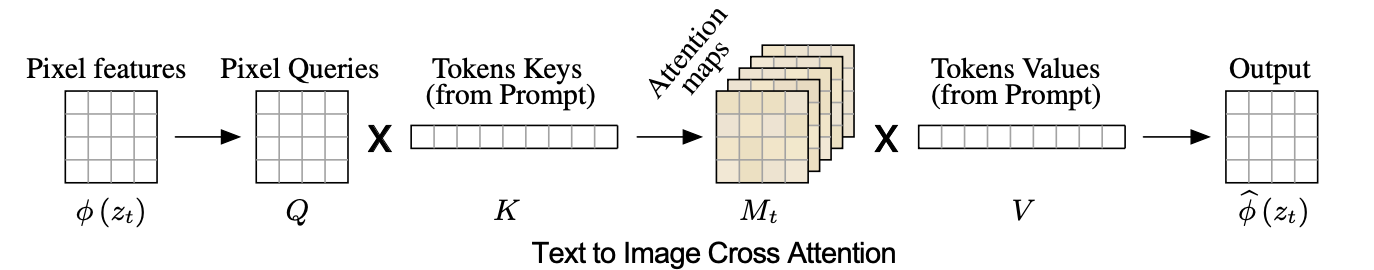
\includegraphics[width=.9\linewidth]{fig/cross_attention.png}
        \caption{Visual and textual embedding are fused using cross-attention layers that produce attention maps for each textual token. Figure source: \href{https://arxiv.org/pdf/2208.01626.pdf}{Hertz et al. (2022)}}
        \label{fig:crossattention}
    \end{figure}

\textbf{Latent Diffusion Model:} 

You will implement the \lstinline{text2image_ldm} method. In that method, we provided some suggested structure by giving you the left-hand side of the initializations. 

Implementing this method requires you to have already read the HuggingFace Diffusers API. See above. You will be working with the \lstinline{DiffusionPipeline} type, but the line \lstinline{DiffusionPipeline.from_pretrained(model_id)} is actually loading a class of type \lstinline{StableDiffusionPipeline}.


Here is an overview of the key steps this method performs:
\begin{itemize}
 
 \item Attention Control Registration: The function begins by registering an attention control mechanism within the model using the provided controller.
 
 \item Tokenization and Embedding of Prompts: The model's tokenizer converts both an empty string (to represent the unconditional generation case) and the actual text prompts into tokenized inputs. These tokenized inputs are then passed through a BERT-like model to obtain embeddings. The embeddings for the unconditional inputs and the text prompts are concatenated to serve as the context for the diffusion process.

(Important note: the particular text encoder we are using has a maximum length of 77 tokens. You will notice this \lstinline{max_len} is fixed to 77 in the starter code.)
 
 \item Latent Space Initialization: It initializes a latent space with the specified dimensions. This space will evolve into the final image through the diffusion process.
 
  \item Diffusion Process: The core of the image generation happens here. For each timestep defined by num\_inference\_steps, the function performs a diffusion step. This involves manipulating the latent space towards the desired outcome based on the context and the current timestep, under the guidance of the specified scale. The controller plays a role here in directing the attention mechanism during these steps.

  \item Image Generation: After completing the diffusion steps, the final latent representation is converted into an image using the model's VQ-VAE (Vector Quantized Variational AutoEncoder).

\end{itemize}

Hint: Some of these steps can be performed simply by utilising the necessary methods from \lstinline{ptp_utils.py}.


\textbf{Cross Attention:} 

The LDM utilizes text prompts to influence the noise prediction at each diffusion step through cross-attention layers. Essentially, at each step $t$, the model predicts noise $\epsilon$ based on a noisy image $z_t$ and the text prompt's embedding $\psi(P)$ using a U-net architecture, leading to the final image $I = z_0$. The key interaction between image and text occurs in the noise prediction phase, where visual and textual embeddings are integrated via cross-attention layers. As illustrated in Fig.~\ref{fig:crossattention}, these layers generate spatial attention maps for textual tokens by projecting the image's deep features and text embedding into query ($Q$), key ($K$), and value ($V$) matrices through learned projections $\ell_Q, \ell_K, \ell_V$. The attention mechanism is formulated as:
\begin{equation}
M = \text{Softmax} \left( \frac{QK^T}{\sqrt{d}} \right),
\end{equation}
where $M_{ij}$ represents the influence of the $j$-th token's value on the $i$-th pixel, with $d_k$ being the dimensionality of the keys and queries. The output from cross-attention, $\phi_b(z_t) = MV$, updates the image features $\phi(z_t)$. Intuitively, $MV$ is a weighted average of $V$ based on the attention maps $M$, which are correlated to the similarity between Q and K. This process leverages multi-head attention to enhance expressiveness, concatenating the outcomes from parallel heads and refining them through an additional linear layer for the final output.

\textbf{Controlling Cross Attention:} 

Pixels are more attracted (correlated) to the words that describe them (you will visualize this when you run the notebook).
Building on the insight that cross-attention maps dictate the spatial layout and relationship between pixels and their corresponding descriptive words, Prompt2Prompt proposes a method to edit images while maintaining their original structure. By reusing attention maps $M$ from an initial generation with prompt $P$ in a subsequent generation with an altered prompt $P^*$, we can create an edited image $I^*$ that respects the original image's layout $I$.

We can define $DM(z_t, P, t, s)$ as the function for a single diffusion step $t$, outputting a noisy image $z_{t-1}$ and optionally an attention map $M_t$. We denote $DM(z_t, P, t, s)\{M \leftarrow \hat{M}\}$ to indicate the diffusion step with an externally supplied attention map $\hat{M}$ overriding the attention map \( M \), while maintaining the value matrix $V$ from $P$. The attention map generated with the edited prompt $P^*$ is $M_t^*$. The function $\text{Edit}(M_t, M_t^*, t)$ represents an editing operation on the attention maps of the original and edited prompts at step $t$. This general algo is written out in Fig.~\ref{fig:algo}.

    \begin{figure}[h!]
        \centering
        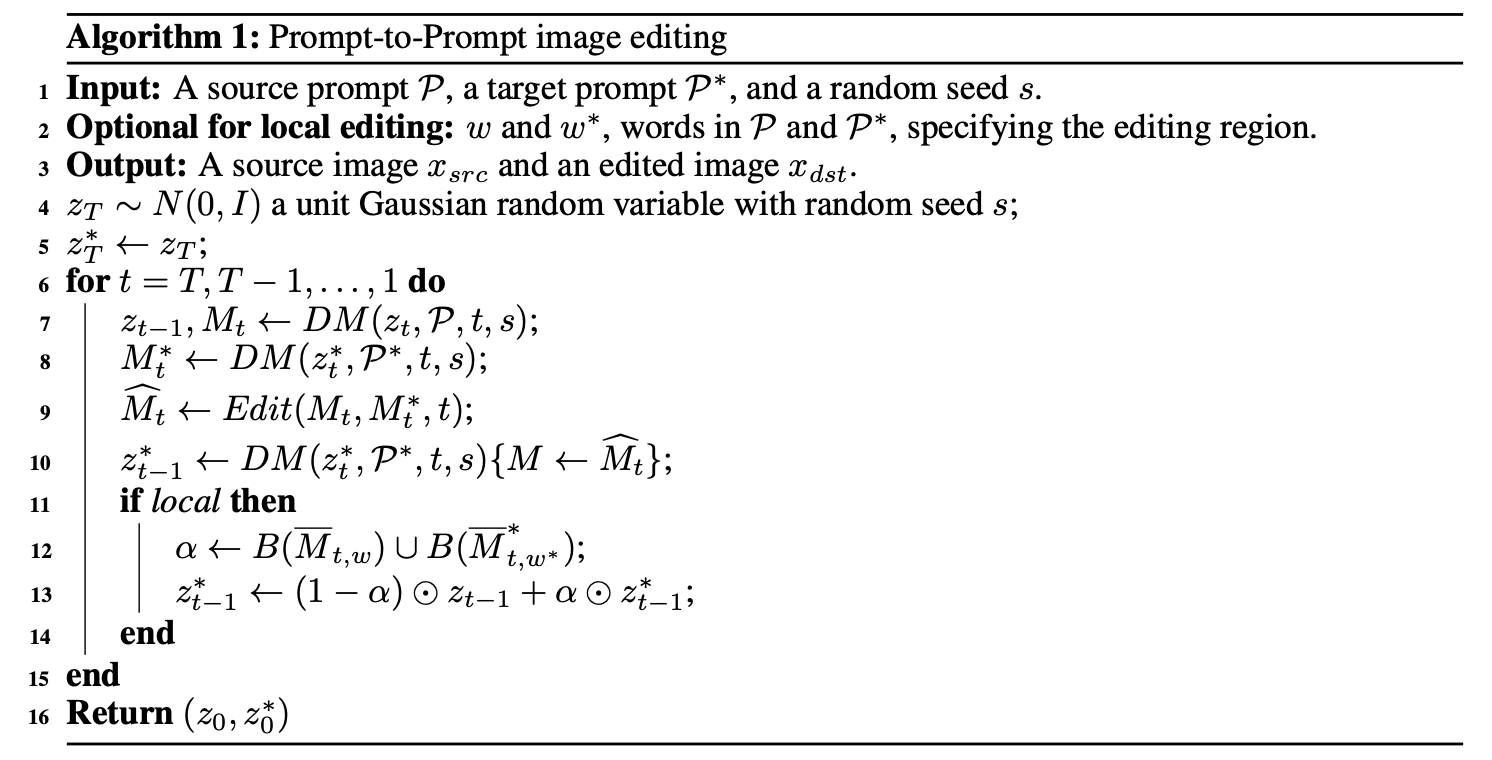
\includegraphics[width=.9\linewidth]{fig/algo.png}
        \caption{Algorithm: Prompt-to-Prompt image editing. Source: \href{https://arxiv.org/pdf/2208.01626.pdf}{Hertz et al. (2022)}. Note that \textit{local} is always False in our implementation. }
        \label{fig:algo}
    \end{figure}

\textbf{Word Swap:} 

While Prompt-to-Prompt can be used for various different types of edit operations on the prompt, we will focus exclusively on word swapping, e.g., \( P\) = “a
big bicycle” to \( P^* \)= “a big car”.

For word swapping, we inject the attention maps of the source image into the generation by the modified prompt. We work with the \lstinline{AttentionReplace} class, where you will initialize a mapper tensor as \lstinline{self.mapper}. It is designed to facilitate the replacement of tokens in the cross-attention map and should be used to reassign attention from the old tokens to the new ones (dive into the code base to see what exactly it does and also refer to the section on Replacement Mapper). You will implement:

\begin{itemize}
 
\item \lstinline{replace_self_attention}: Responsible for replacing the self-attention map of the current step with the base attention map \lstinline{attn_base} or keeping it unchanged based on the size of the attention map to be replaced \lstinline{att_replace}. This decision is made by comparing the size of the \lstinline{att_replace} with a predefined threshold (in this case, 16 ** 2). If the size is smaller, it expands the \lstinline{attn_base} to match the dimensions of \lstinline{att_replace}; otherwise, it simply returns \lstinline{att_replace}.
 
\item \lstinline{replace_cross_attention}: 
The cross-attention replacement involves a computation that maps the base attention \lstinline{attn_base} through a transformation \lstinline{self.mapper} to produce a new attention map. This transformation aligns the attention from the source domain (tokens from the original prompt) to the target domain (edited image features). 

(Hint: You can accomplish this through careful use of \lstinline{einsum}!)
  
\item \lstinline{forward} method: Algorithm is indicated below:

\begin{center}
    \begin{minipage}{.8\linewidth}
    \begin{algorithm}[H]
    \caption{Forward method of AttentionReplace class}\label{alg:hw4_edit_forward}
        \begin{algorithmic}[1]
            \If {the layer is cross attention layer or the current step is subject to be edited}
                \State Calculate the number of heads $h$
                \State Reshape \lstinline{attn} to be the correct shape
                \State Split \lstinline{attn} to \lstinline{attn_base} and \lstinline{attn_replace}
                
                (\lstinline{attn_base} is the attention for reference example and \lstinline{attn_replace} is the attention for the remaining examples)
                \If {the layer is cross attention layer}
                    \State Edit \lstinline{attn[1:]} with replace cross attention method according to the current step's $\alpha$ (indicating whether to replace the attention for that word) of each individual word
                \Else{}
                    \State Edit \lstinline{attn[1:]} with replace self attention method
                \EndIf
                \State Reshape \lstinline{attn} to be the correct shape
            \EndIf
            \Return \lstinline{attn}
        \end{algorithmic}
    \end{algorithm}
    \end{minipage}
    \end{center}
    \vspace{1em}

(Hint: To see some examples of how the alphas are constructed, you can run the main at the bottom of \lstinline{ptp_utils.py}, e.g. \lstinline{python ptp_utils.py}.)

\end{itemize}


\textbf{Replacement Mapper:}

In the function \lstinline{get_replacement_mapper}, we return the stacked PyTorch tensor containing all the mapping matrices, where each matrix corresponds to the mapping from the first prompt to one of the subsequent prompts. It calls upon \lstinline{get_replacement_mapper_} (which you will implement) that splits both input strings \lstinline{x} and \lstinline{y} into words and constructs a mapping matrix of size \lstinline{max_len} $\times$ \lstinline{max_len}, with values in $[0,1]$ indicating the matching between the changing word in the input prompt and the corresponding word in the modification prompt.

(Hint: For most things in PyTorch we avoid for loops, but you needn't do so here. Since this method is only called once during initialization, for loops are fine.)

(Hint: Use the main at the bottom of \lstinline{seq_aligner.py} to check that your implementation of \lstinline{get_replacement_mapper_} is behaving as expected, e.g. \lstinline{python seq_aligner.py}.)

\textbf{Evaluation:} 

We ask you to run the notebook to get the visualizations once you complete filling in the needed functions. You will be visualizing replacement edit and local editing results.

\clearpage

\uplevel{\subsection*{Empirical Questions}}

The questions below refer directly to the section headers of the Colab notebook in \lstinline{run_in_colab.ipynb}.

\begin{parts}

\part[4] Paste the results from the section `Baseline: Cross-Attention Visualization'

[Expected runtime on Colab T4: 10s]

\begin{answer_box}[title=,height=8cm, width=15cm]
  \end{answer_box}


\part[3] Briefly explain what the greyscale cross-attention visualization reveals to you about the behavior of the model.

\begin{answer_box}[title=,height=8cm, width=15cm]
\end{answer_box}


\clearpage
\part[4] Paste the results from the section `Baseline: No Attention Controller'
\label{question-baseline}

[Expected runtime on Colab T4: 30s]

\begin{answer_box}[title=,height=8cm, width=15cm]
  \end{answer_box}
  
\part[4] Paste the results from the section `Prompt-to-Prompt: Word-swap'
\label{question-a}

[Expected runtime on Colab T4: 30s]

\begin{answer_box}[title=,height=8cm, width=15cm]
  \end{answer_box}

\clearpage
\part[1] Briefly explain how your results from Question \ref{question-baseline} differ from your results in Question \ref{question-a}?

\begin{answer_box}[title=,height=5cm, width=15cm]
\end{answer_box}

\part[4] Paste the results from the section `Prompt-to-Prompt: Modify Cross-Attention injection'
\label{question-b}

[Expected runtime on Colab T4: 30s]

\begin{answer_box}[title=,height=12cm, width=15cm]
  \end{answer_box}

\clearpage

\part[2] How do you your results in Question \ref{question-b} vary as you change the word-specific cross attention parameters? 

\begin{answer_box}[title=,height=4cm, width=15cm]
\end{answer_box}

\part[4] Paste the results from the section `Prompt-to-Prompt: Local Edit'
\label{question-c}

[Expected runtime on Colab T4: 30s]

\begin{answer_box}[title=,height=8cm, width=15cm]
  \end{answer_box}


\part[2] Intuitively, what do we accomplish by setting \lstinline{"default_": 1.} and a word specific attention parameter to a much smaller value, e.g. \lstinline{"lasagne": .2}, in Question \ref{question-c}? 

\begin{answer_box}[title=,height=4cm, width=15cm]
\end{answer_box}


\clearpage
\part Define your own base prompt and three prompt edits (i.e. something other than the examples provided in the \lstinline{.ipynb}) and run them through Prompt-to-Prompt.

\begin{subparts}

\subpart[1] Report the prompts and any hyperparameters that you used.
\begin{answer_box}[title=,height=8cm, width=15cm]
  \end{answer_box}
  
\subpart[2] Paste the resulting images below.
\begin{answer_box}[title=,height=8cm, width=15cm]
  \end{answer_box}
     
\end{subparts}


  
\end{parts}


\clearpage
\sectionquestion{Code Upload}

\begin{parts}

\part[0] Did you upload your code to the appropriate programming slot on Gradescope? \\
\emph{Hint:} The correct answer is `yes'.

    \begin{checkboxes}
     \choice Yes 
     \choice No
    \end{checkboxes}

For this homework, you should upload all the code files that contain your new and/or changed code. Files of type \lstinline{.py} and \lstinline{.ipynb} are both fine.

\end{parts}

\newpage
\sectionquestion{Collaboration Questions}

\begin{parts}

\uplevel{After you have completed all other components of this assignment, report your answers to these questions regarding the collaboration policy. Details of the policy can be found in the syllabus.}

    \part[1] Did you collaborate with anyone on this assignment? If so, list their name or Andrew ID and which problems you worked together on.

        \begin{answer_box}[title=,height=3cm, width=15cm]
        \end{answer_box}

    
    \part[1] Did you find or come across code that implements any part of this assignment? If so, include full details.
        \begin{answer_box}[title=,height=3cm, width=15cm]
        \end{answer_box}
\end{parts}
\end{questions}


\end{document}
